\def\QRCODE{TB_image_TUT.IMG.machine_learning_matlabqrcode.png}
\def\QRPAGE{http://www.iptutorials.science/tree/master/TB_image/TUT.IMG.machine_learning/matlab}
\mcorrectionsection{Matlab correction}

\subsection{Feature extraction}
We make a loop on the whole database to extract some features of each image. The 9 features used here are: area, convex area, eccentricity, equivalent diameter, extent, major axis length, minor axis length, perimeter and solidity. All these parameters are defined in the documentation of the Matlab function \minline{regionprops}.

\begin{matlab}
% 18 classes of 12 images
folderImages = './images_Kimia216/';
classes = {'bird','bone','brick','camel','car','children',...
    'classic','elephant','face','fork','fountain',...
    'glass','hammer','heart','key','misk','ray','turtle'};
nbClasses = length(classes);
nbImages = 12;

features = [];
targets = zeros(nbClasses,nbClasses*nbImages);

for i=1:nbClasses
    for k=1:nbImages
        nameImage = strcat(folderImages,classes{i},'-',num2str(k),'.bmp');
        currentImage = imread(nameImage);
        currentImage = currentImage==0;
        s  = regionprops(currentImage,'Area','ConvexArea',...
            'Eccentricity','EquivDiameter','Extent',...
            'MajorAxisLength','MinorAxisLength',...
            'Perimeter','Solidity');
        sArray = [s.Area;s.ConvexArea;s.Eccentricity;...
            s.EquivDiameter;s.Extent;...
            s.MajorAxisLength;s.MinorAxisLength;...
            s.Perimeter;s.Solidity];
        features = [features,sArray(:,1)];       
    end
    targets(i,(i-1)*nbImages+[1:nbImages]) = 1;
end
\end{matlab}

Note that in the same time, the target array (required in the following) is built within this loop. It represents the true classes of the objects.

\subsection{Classification}
The network is created with 10 hidden layers. We used a training set of $75\%$ of the database and $25\%$ for the test set.

\begin{matlab}
% create the network
hiddenLayerSize = 10;
net = patternnet(hiddenLayerSize);

% set up the division of data
net.divideParam.trainRatio = 75/100;
%net.divideParam.valRatio   = 20/100;
net.divideParam.testRatio  = 25/100;
\end{matlab}

Now the network is trained and tested:

\begin{matlab}
% train the network
[net,tr] = train(net,features,targets);

% test the network
outputs = net(features);
\end{matlab}

The overall performance as well as the confusion matrix is here computed:

\begin{matlab}
% overall performance
[c,cm,ind,per] = confusion(targets,outputs);
perf = 1-c

% confusion matrix
figure; plotconfusion(targets,outputs);
\end{matlab}

and the result is:
\begin{mwindow}
perf =  0.9444
\end{mwindow}

\begin{figure}[htbp]
\centering
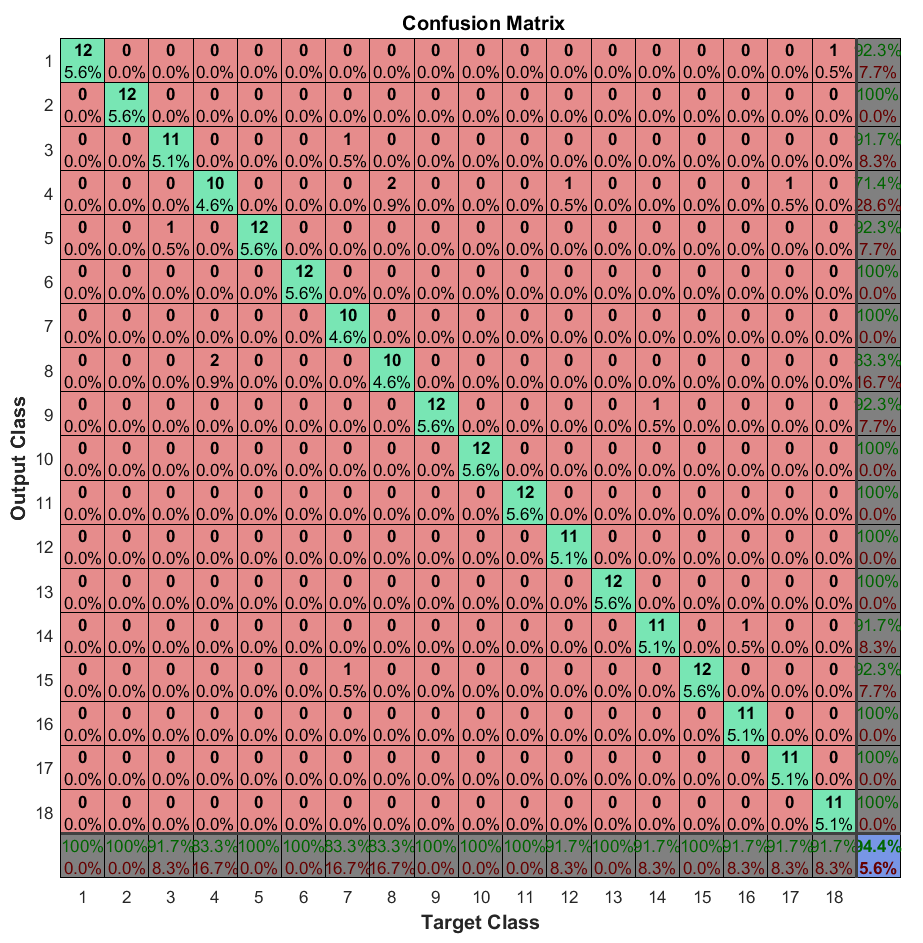
\includegraphics[width=\linewidth]{confusion.png}
\caption{Confusion matrix of the classification result.}
 \label{fig:machine_learning:matlab:confusion}
\end{figure}

Note that if we run the same code, the result can be different since the initialization of the optimization process (used for the training task) is different.\\
For example, by running again, we get the following result:
\begin{mwindow}
perf =  0.9167
\end{mwindow}
